%=======================================================================
%  3.3 CONCEPT EVALUATION & ITERATION  (text from the Word report; audit edits only)
%=======================================================================
\needspace{24\baselineskip}
\subsection{Concept Evaluation \& Iteration}
\label{sec:evaluation}

\subsubsection{Comparison against the KPIs}
\label{sec:kpicompare}

Table~\ref{tab:kpicompare} compares the concepts against the KPIs of
Table~\ref{tab:kpi} using the estimates from Sections~\ref{sec:check1},
\ref{sec:check2} and \ref{sec:conceptB}; no surface-temperature reduction has been
calculated. Each rating is on a 1--5 scale and carries its reason; an unrated KPI is
a gap in evidence and does not count as zero.

\begin{table}[!htb]
\centering
\caption{KPI comparison using preliminary engineering estimates. Ratings 1--5;
\enquote{--} means no evidence yet.}
\label{tab:kpicompare}
\renewcommand{\arraystretch}{1.15}
\small
\begin{tabularx}{\textwidth}{L{2.6cm} X X}
\toprule
\textbf{KPI (unit)} & \textbf{A V1 --- water façade} & \textbf{B V1 --- roughness spray} \\
\midrule
KPI1 solar reflectance (--) &
  Roof: 0.95 assumed. \textbf{4}: high value, but assumed and only on the roof. &
  Not specified. \textbf{2}: no reflective function is designed in. \\
KPI2 shaded share of the façade (\%) &
  Fins added; duration not calculated. \textbf{3}: the function is present, the number is missing. &
  \qty{0}{\percent} added by the coating. \textbf{1}. \\
KPI3 heat removed (\si{\kilo\watt}; \si{\watt\per\square\metre}) &
  \qty{740}{\square\metre} roof: $\approx$\qtyrange{30}{62}{\kilo\watt} across benchmark / cooler-sky cases; $\approx$\qtyrange{3}{22}{\kilo\watt} for warmer sky. \textbf{4}: estimated, roof-limited. &
  About \qty{12}{\kilo\watt} by the order-of-magnitude estimate of Section~\ref{sec:conceptB}; released into the canyon air, and the sign is uncertain at low wind. \textbf{2}. \\
Heat transport (\si{\kilo\watt}; \si{\kilo\gram\per\second}) &
  \qty{122}{\kilo\watt} assumed load requires \qty{2.9}{\kilo\gram\per\second} at \qty{10}{\celsius} difference or \qty{9.7}{\kilo\gram\per\second} at \qty{3}{\celsius}. &
  Local exchange; rate not quantified. \\
KPI4 surface temperature reduction (\si{\kelvin}) &
  Not calculated. \textbf{--} &
  Not calculated. \textbf{--} \\
KPI5 water consumed (\si{\litre\per\square\metre\per\day}) &
  0 in normal operation; filling and leakage are separate. \textbf{5}. &
  0 for a dry coating. \textbf{5}. \\
KPI6 performance retained (\%) &
  No ageing data. \textbf{--} &
  No ageing data. \textbf{--} \\
\midrule
Sum of rated KPIs (max.\ 20) & \textbf{16} & \textbf{10} \\
\bottomrule
\end{tabularx}
\end{table}

The flow rates are requirements that the circulation check has to meet. Even the
highest roof estimate is below the assumed \qty{122}{\kilo\watt} load.

\subsubsection{Engineering Review and Selection}
\label{sec:review}

We reviewed both V1 concepts in the team and with an AI assistant as critical
reviewer; the tool is declared in Appendix~A. Table~\ref{tab:review} lists the
issues raised, our response and the resulting decision.

\begin{table}[!htb]
\centering
\caption{Team review and critical assessment of AI feedback.}
\label{tab:review}
\renewcommand{\arraystretch}{1.15}
\small
\begin{tabularx}{\textwidth}{L{4.0cm} L{1.8cm} X}
\toprule
\textbf{Review issue} & \textbf{Response} & \textbf{Resulting decision} \\
\midrule
Pipes hidden behind the absorber risk hidden damage & Accept & Move pipes into a separate external layer; enable access and retrofit. \\
Roof area and resistance limit \textbf{A} & Accept & Limit connected area; use larger mains and short parallel circuits. \\
Weak ventilation rules out \textbf{B} & Qualify & Airflow is uncertain, but texture does not automatically fail. Test its mechanism. \\
Existing KPI definitions are incomplete & Accept & Use heat-flow units; define targets and test conditions before measurement. \\
\bottomrule
\end{tabularx}
\end{table}

Reduced air exchange in Modellierungsgebiet 03 makes B's airflow-dependent benefit
uncertain~\cite[pp.~148--151]{stadtzuerich2020}, \cite{blocken2009}. Elephant hairs
can aid heat transfer at low wind, whereas transverse wooden ribs reduced natural
convection in another study~\cite{myhrvold2012,ahmed2024}.

\textbf{A} was selected because it combines shading with heat transport to a
separate release surface, and because B's benefit is not demonstrated
(Table~\ref{tab:kpicompare}).

\subsubsection{Final Concept V2 --- Construction and Heat Paths}
\label{sec:v2}

V2 moves the pipes into separable panels outside the original wall, allowing both
new construction and retrofit. The wall is retained apart from mounting connections.
A small gap behind the added layer is intended to let escaped water fall away
externally, reducing hidden wall-damage risk without guaranteeing leak-proof
protection (Figure~\ref{fig:v2sections}).

\begin{figure}[htbp]
\centering
\begin{minipage}[t]{0.42\textwidth}
\centering
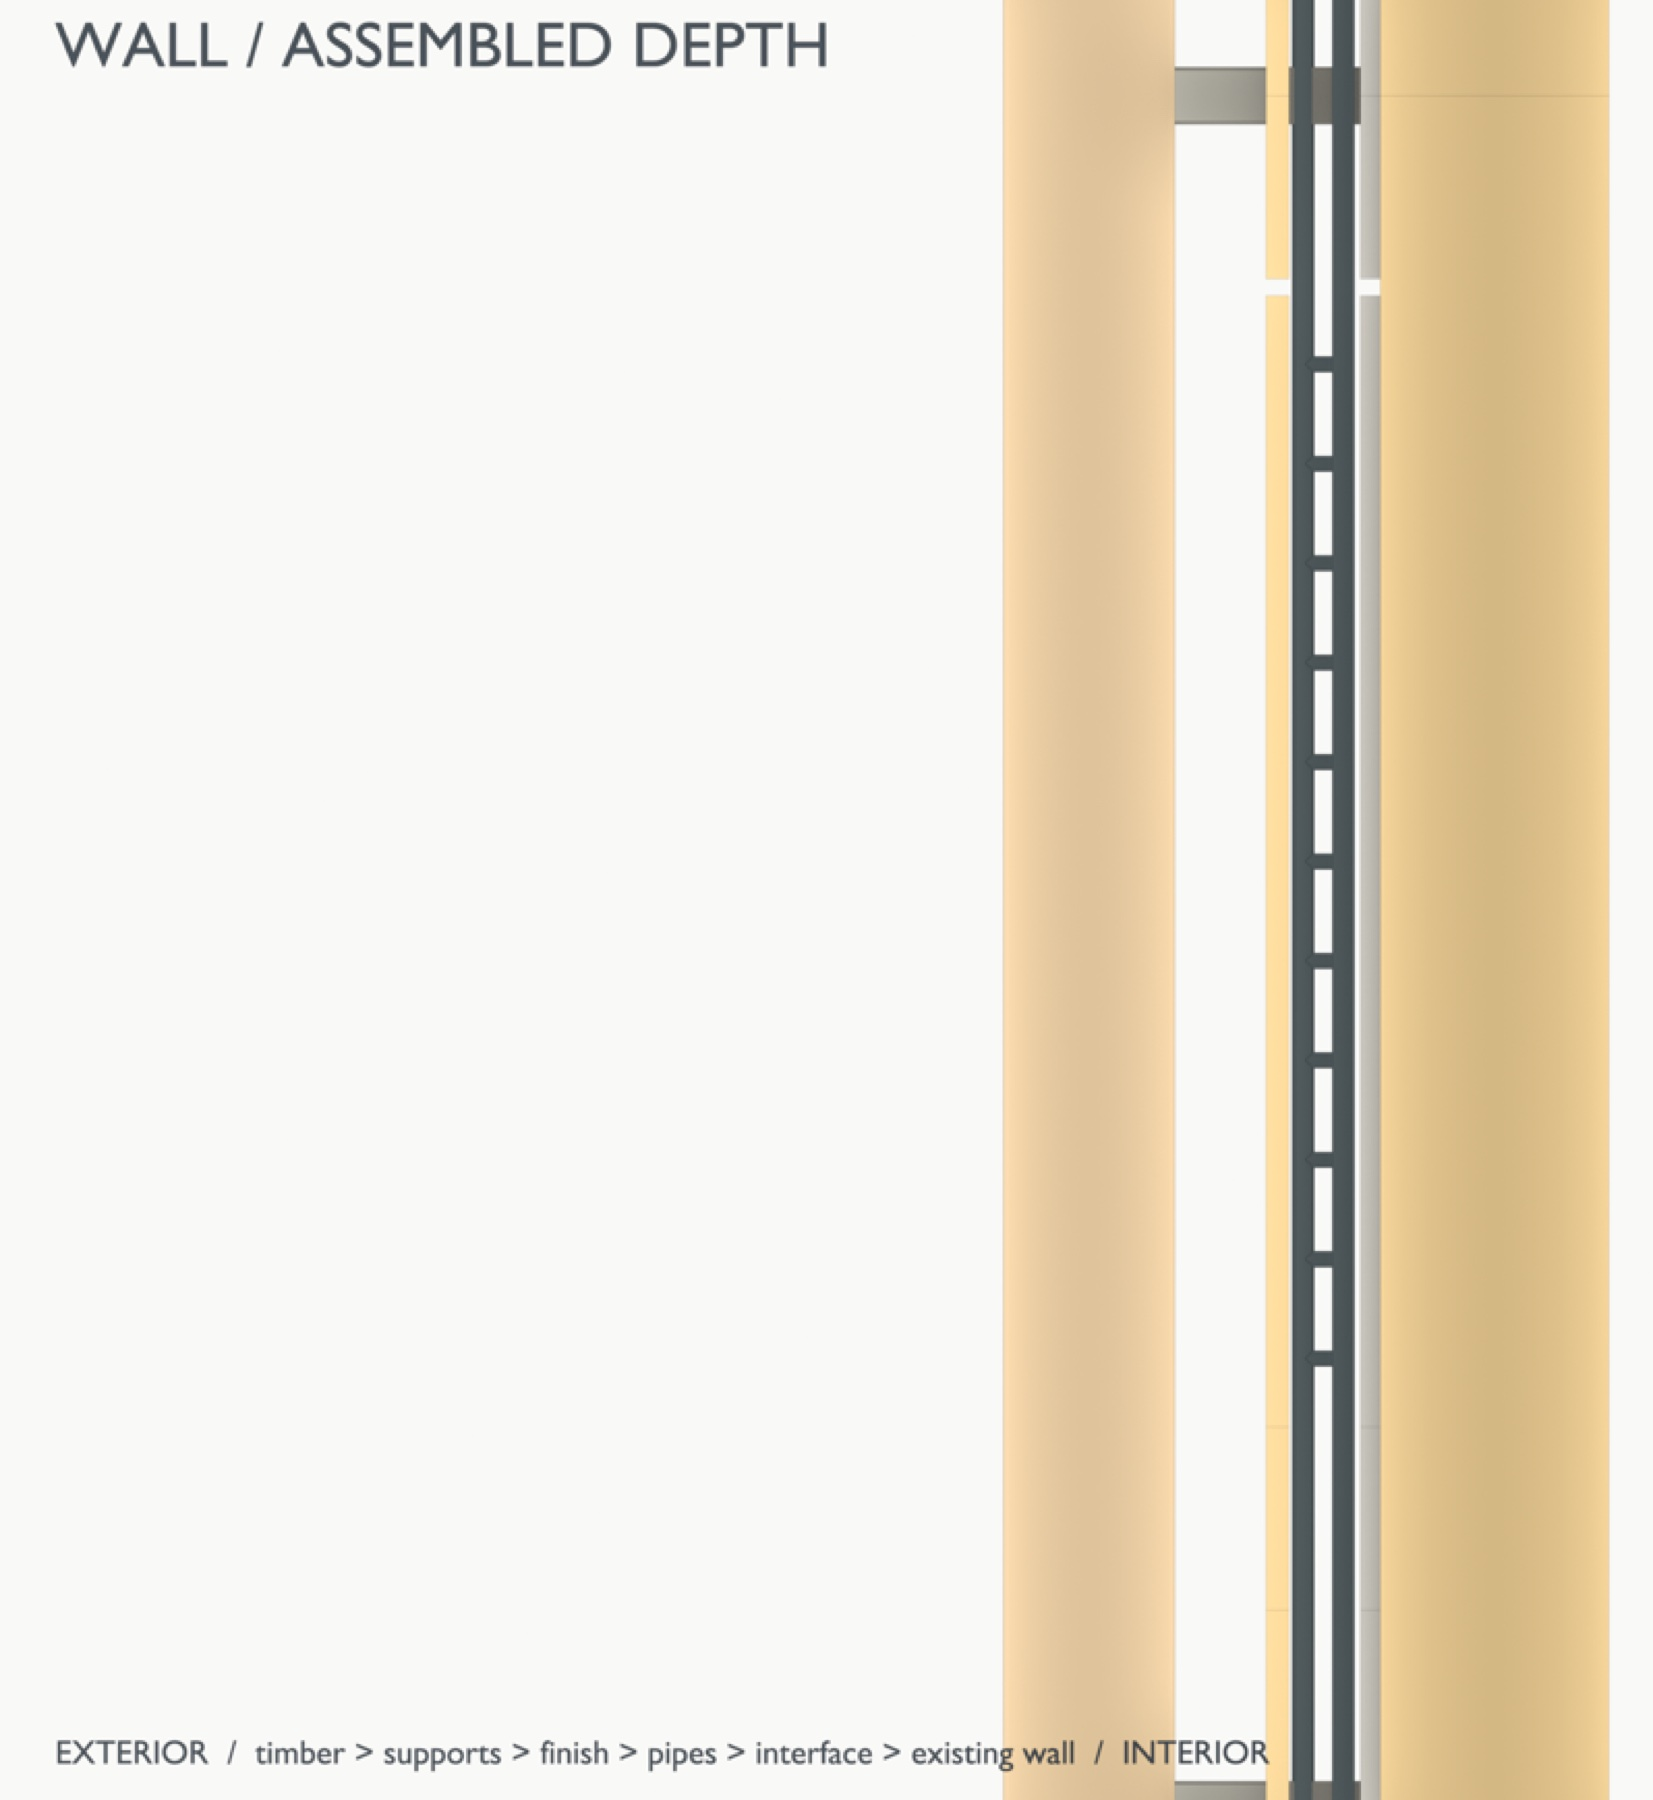
\includegraphics[width=\linewidth]{figures/image10.jpg}
\end{minipage}\hfill
\begin{minipage}[t]{0.54\textwidth}
\centering
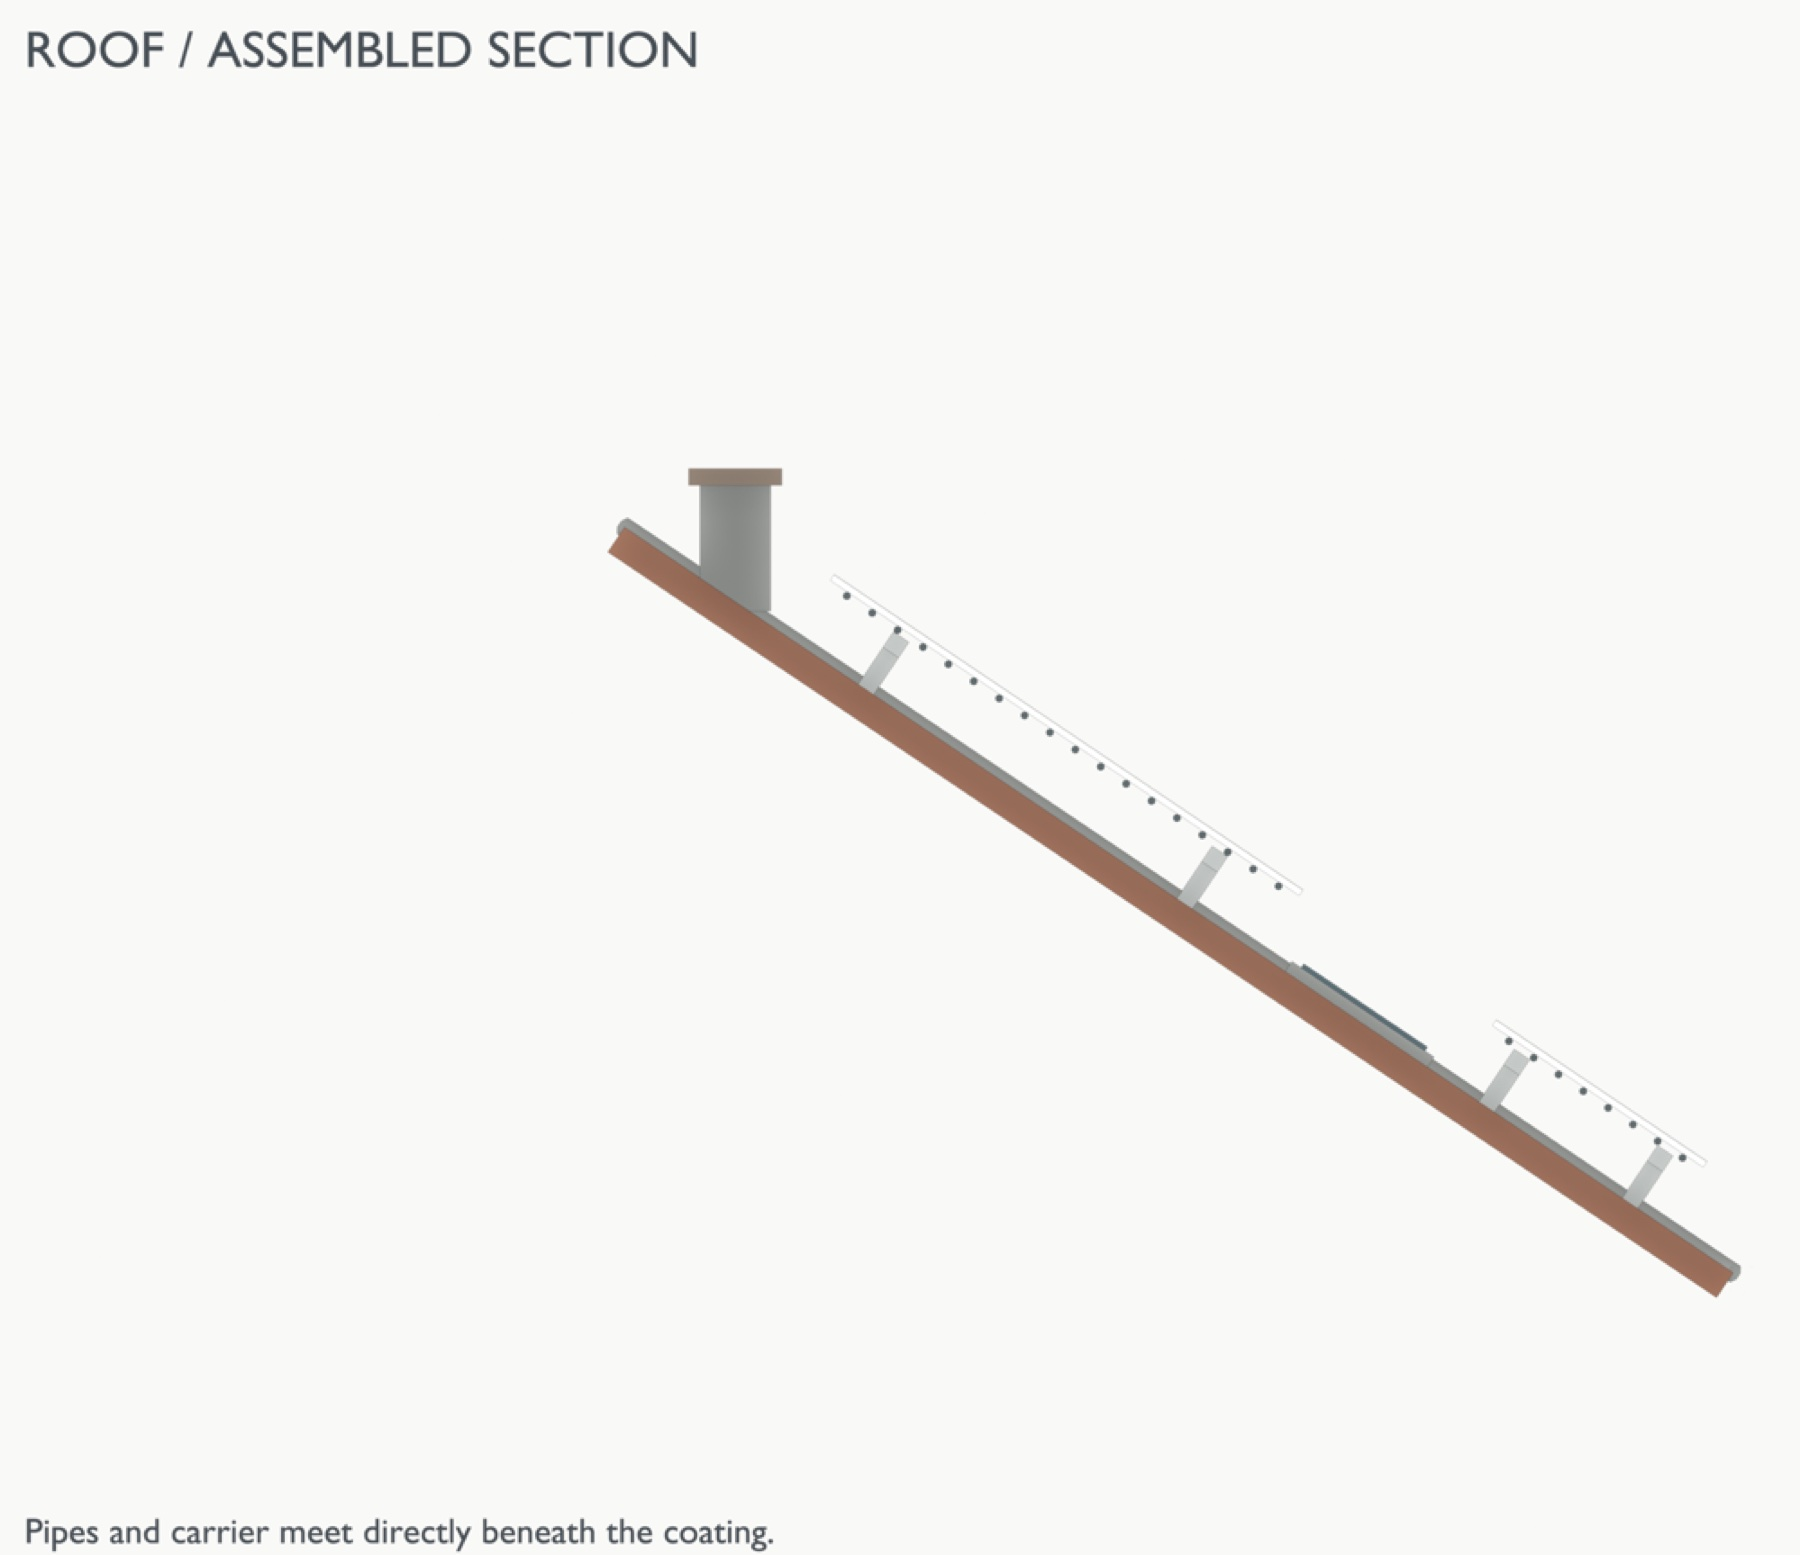
\includegraphics[width=\linewidth]{figures/image11.jpg}
\end{minipage}
\caption{Our assembled sections. Façade, outside inward: timber ribs, supports/air
space, collector panel, pipes, interface, existing wall. Roof: coating, carrier
plate, pipes, supports, existing roof. Render: project team.}
\label{fig:v2sections}
\end{figure}

Heat passes from the façade panel into water, then from the roof pipes into the
carrier plate and coated surface. The Saharan silver ant inspires solar reflection
and infrared emission~\cite{shi2015}; the assumed \qty{95}{\percent} reflectance
still needs material verification. No increase in convection is assumed; convective
heat release requires a surface warmer than the air (Figure~\ref{fig:v2loop}).

\begin{figure}[htbp]
\centering
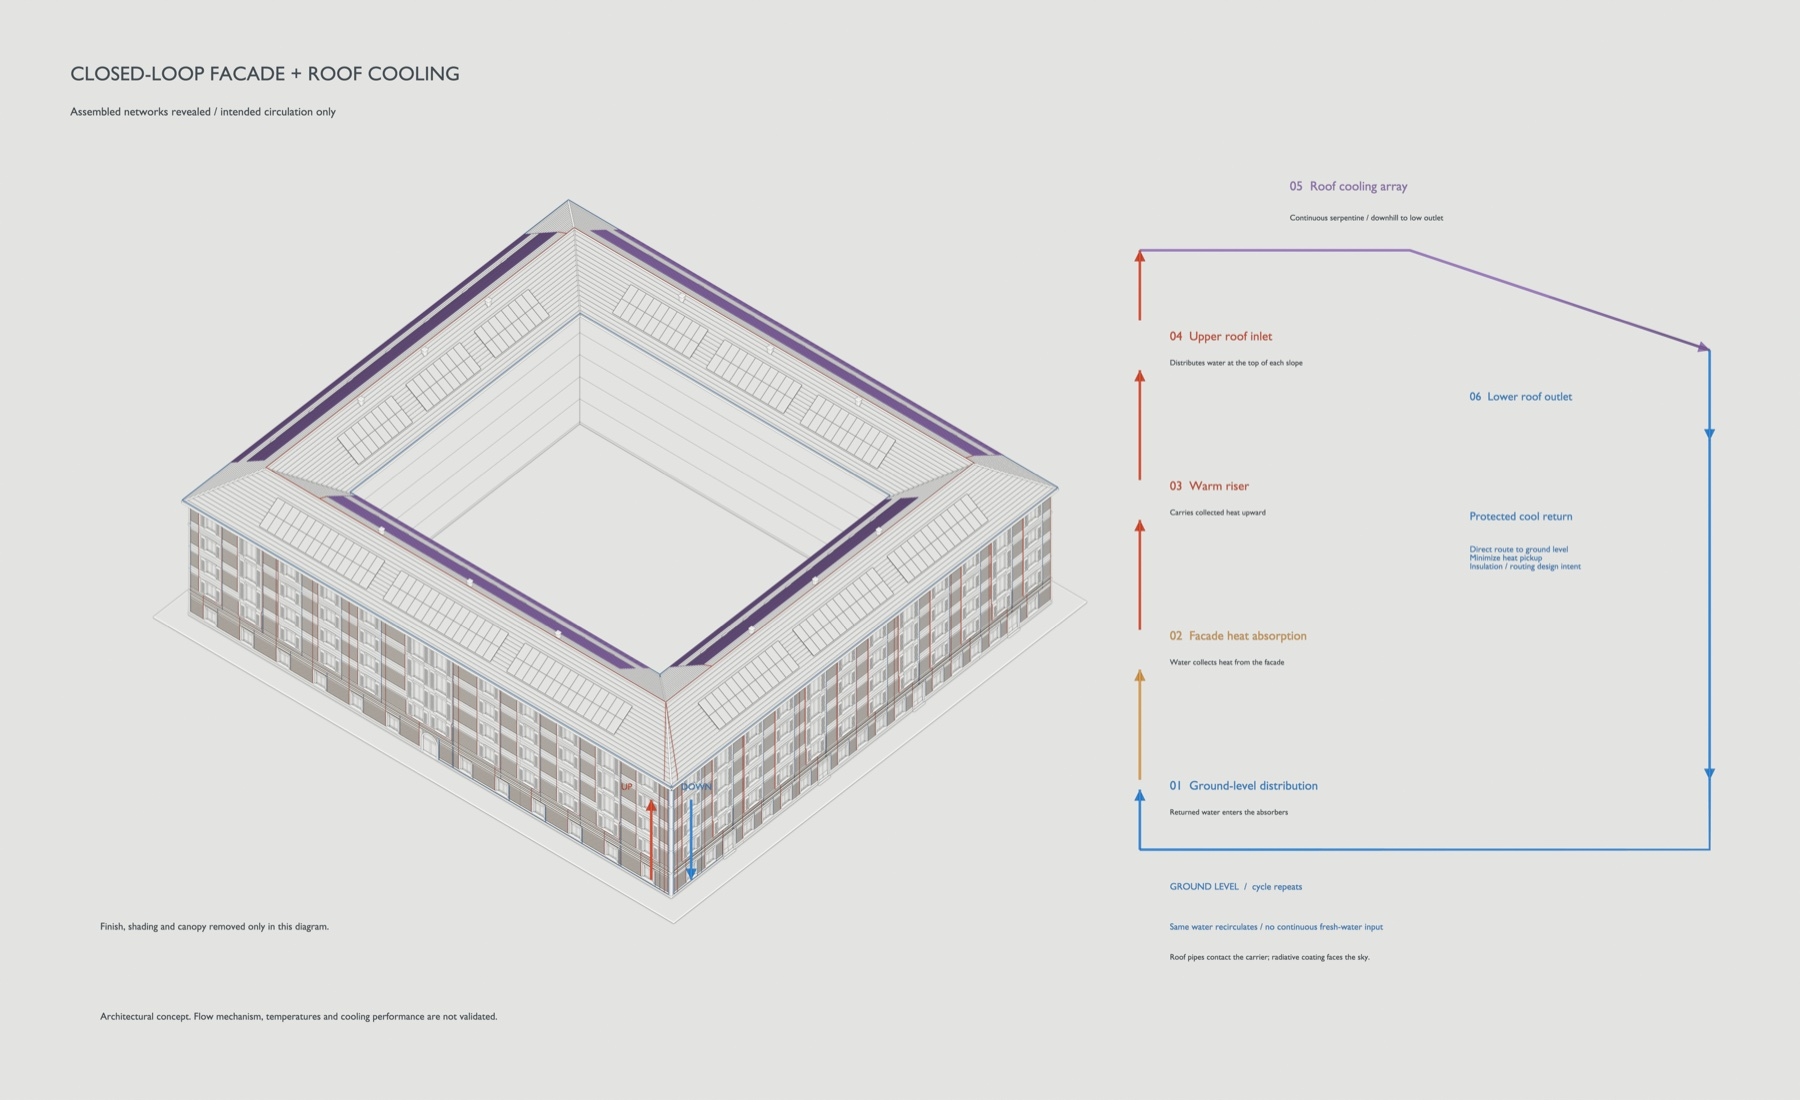
\includegraphics[width=0.85\textwidth]{figures/image12.jpg}
\caption{Intended heat-transfer loop: façade collection $\rightarrow$ warm riser
$\rightarrow$ roof heat release $\rightarrow$ cool return. Render: project team.}
\label{fig:v2loop}
\end{figure}

\subsubsection{Pedestrian Space and Maintenance Access}
\label{sec:v2access}

Compared with V1, we cut back the timber fins to start at the first floor, about
\qty{3.4}{\metre} above ground (Figure~\ref{fig:v2fins}). A new building could set
its wall back to accommodate the fins; this retrofit must retain the wall beside the
pavement. Reducing the modelled ground-floor projection from \qty{0.66}{\metre} to
\qty{0.20}{\metre} leaves \qty{0.46}{\metre} more space.

\begin{figure}[htbp]
\centering
\begin{minipage}[t]{0.48\textwidth}
\centering
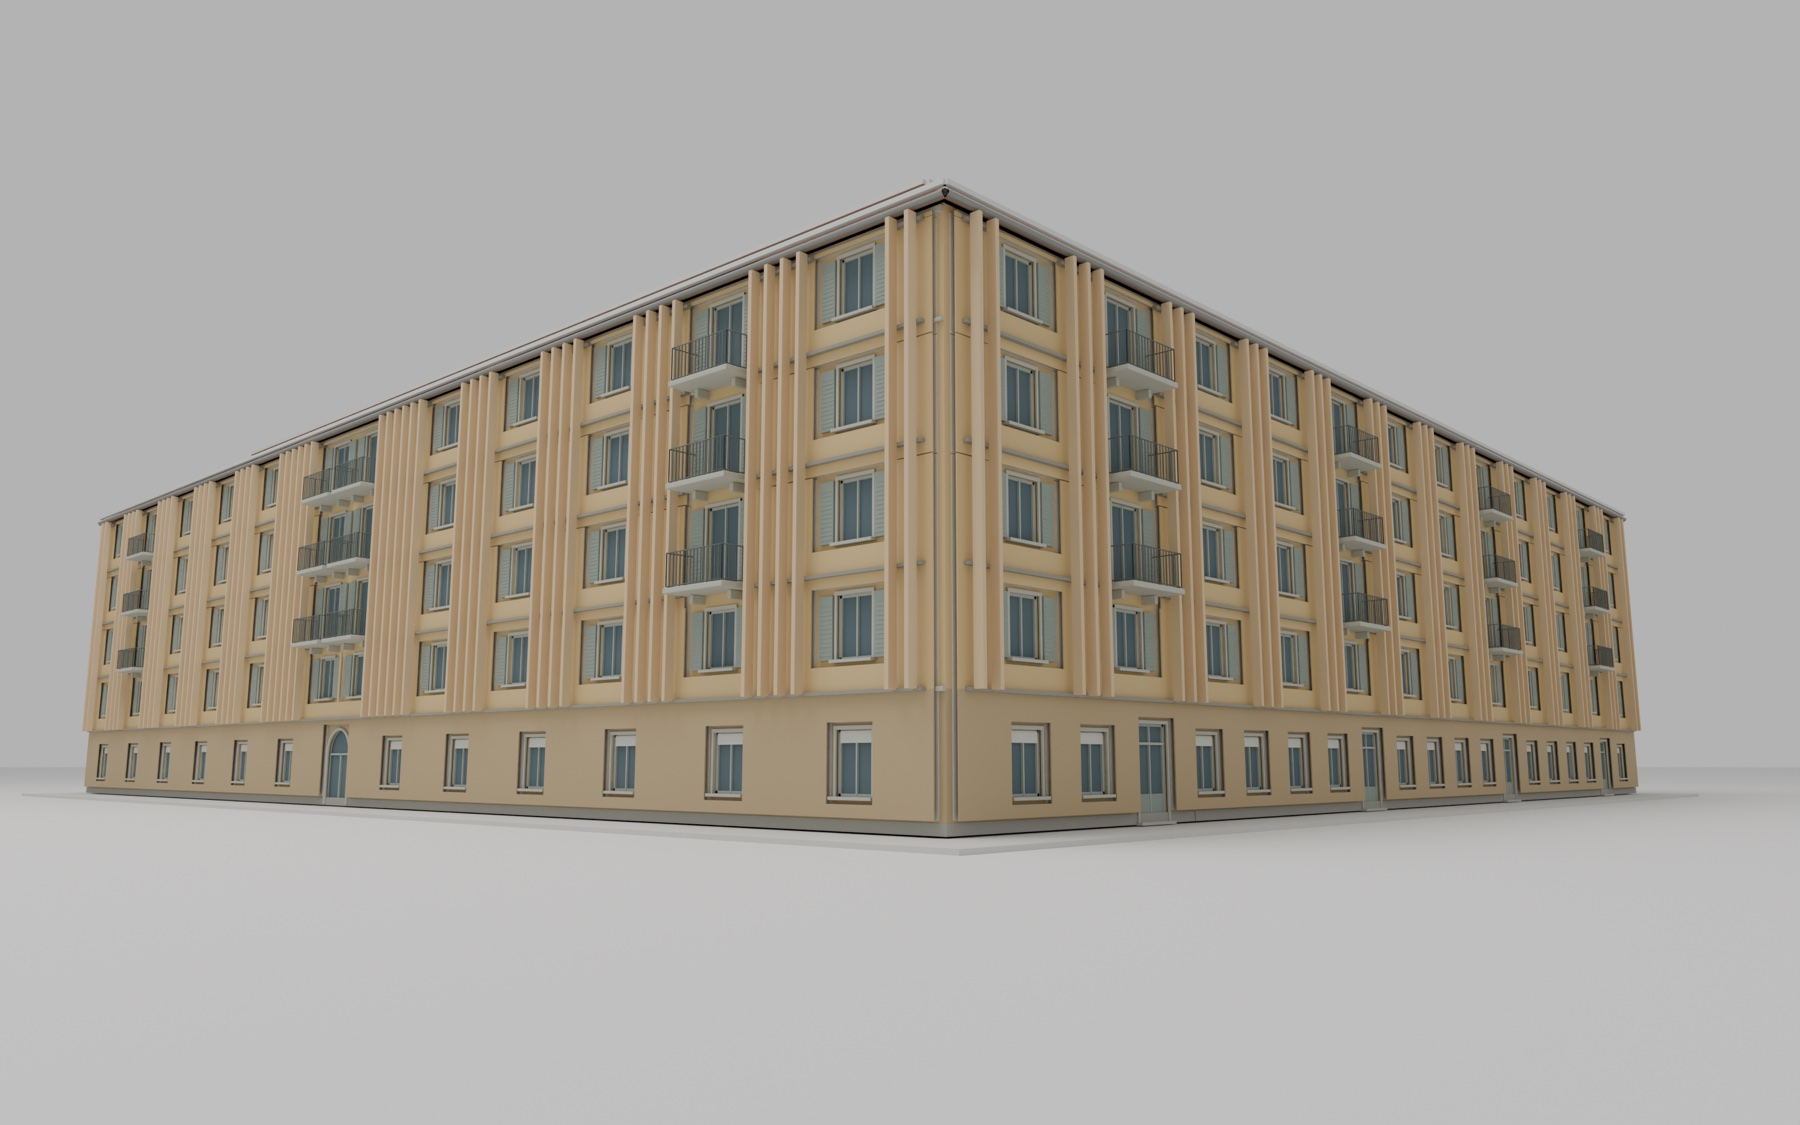
\includegraphics[width=\linewidth]{figures/image13.jpg}\\[1mm]
{\small (a) Fins start at the first floor}
\end{minipage}\hfill
\begin{minipage}[t]{0.48\textwidth}
\centering
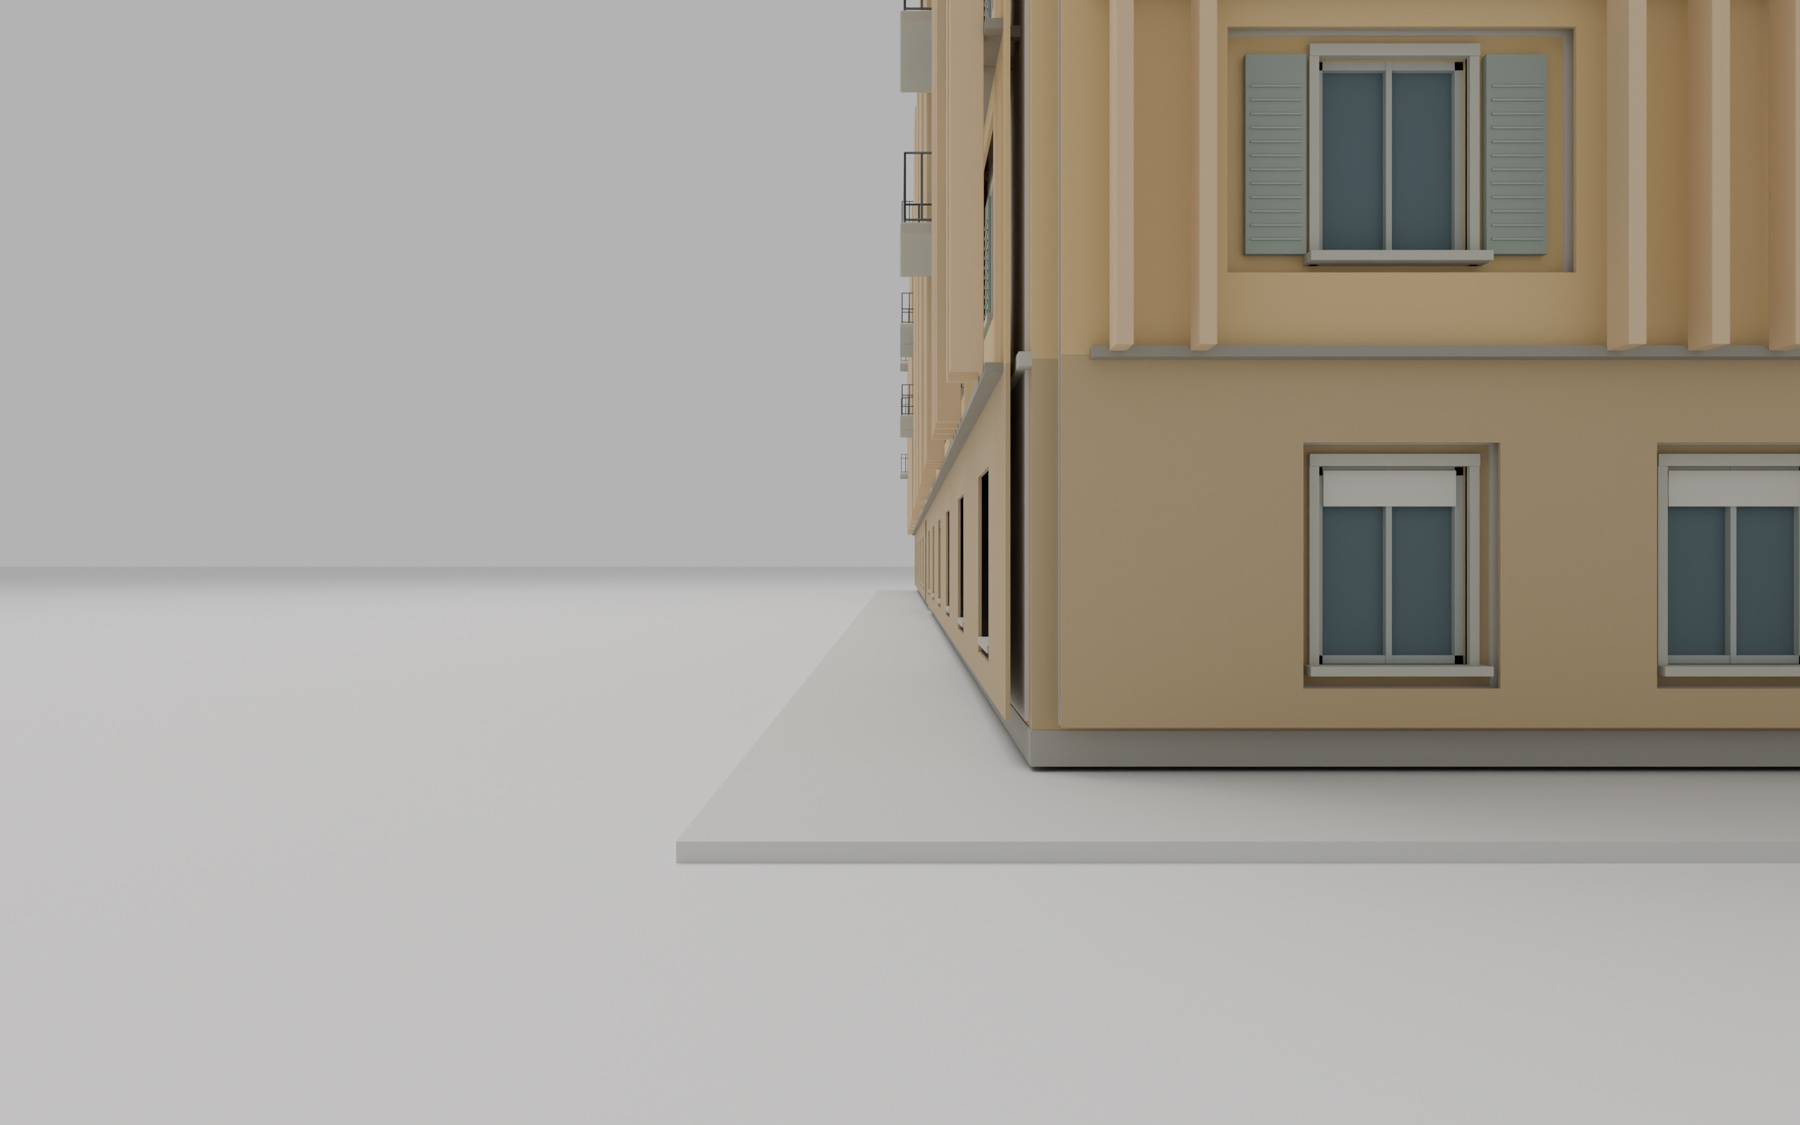
\includegraphics[width=\linewidth]{figures/image14.jpg}\\[1mm]
{\small (b) Thinner base beside the pavement}
\end{minipage}
\caption{Revised timber fins and pedestrian space in our model. Dimensions are
design estimates. Render: project team.}
\label{fig:v2fins}
\end{figure}

Removing individual panels exposes the pipes for inspection and repair without
opening the original wall (Figure~\ref{fig:v2access}). This improves access compared
with V1's hidden pipes. Rib spacing, winter gains and the material checks are taken up
in Section~\ref{sec:benefits}.

\begin{figure}[htbp]
\centering
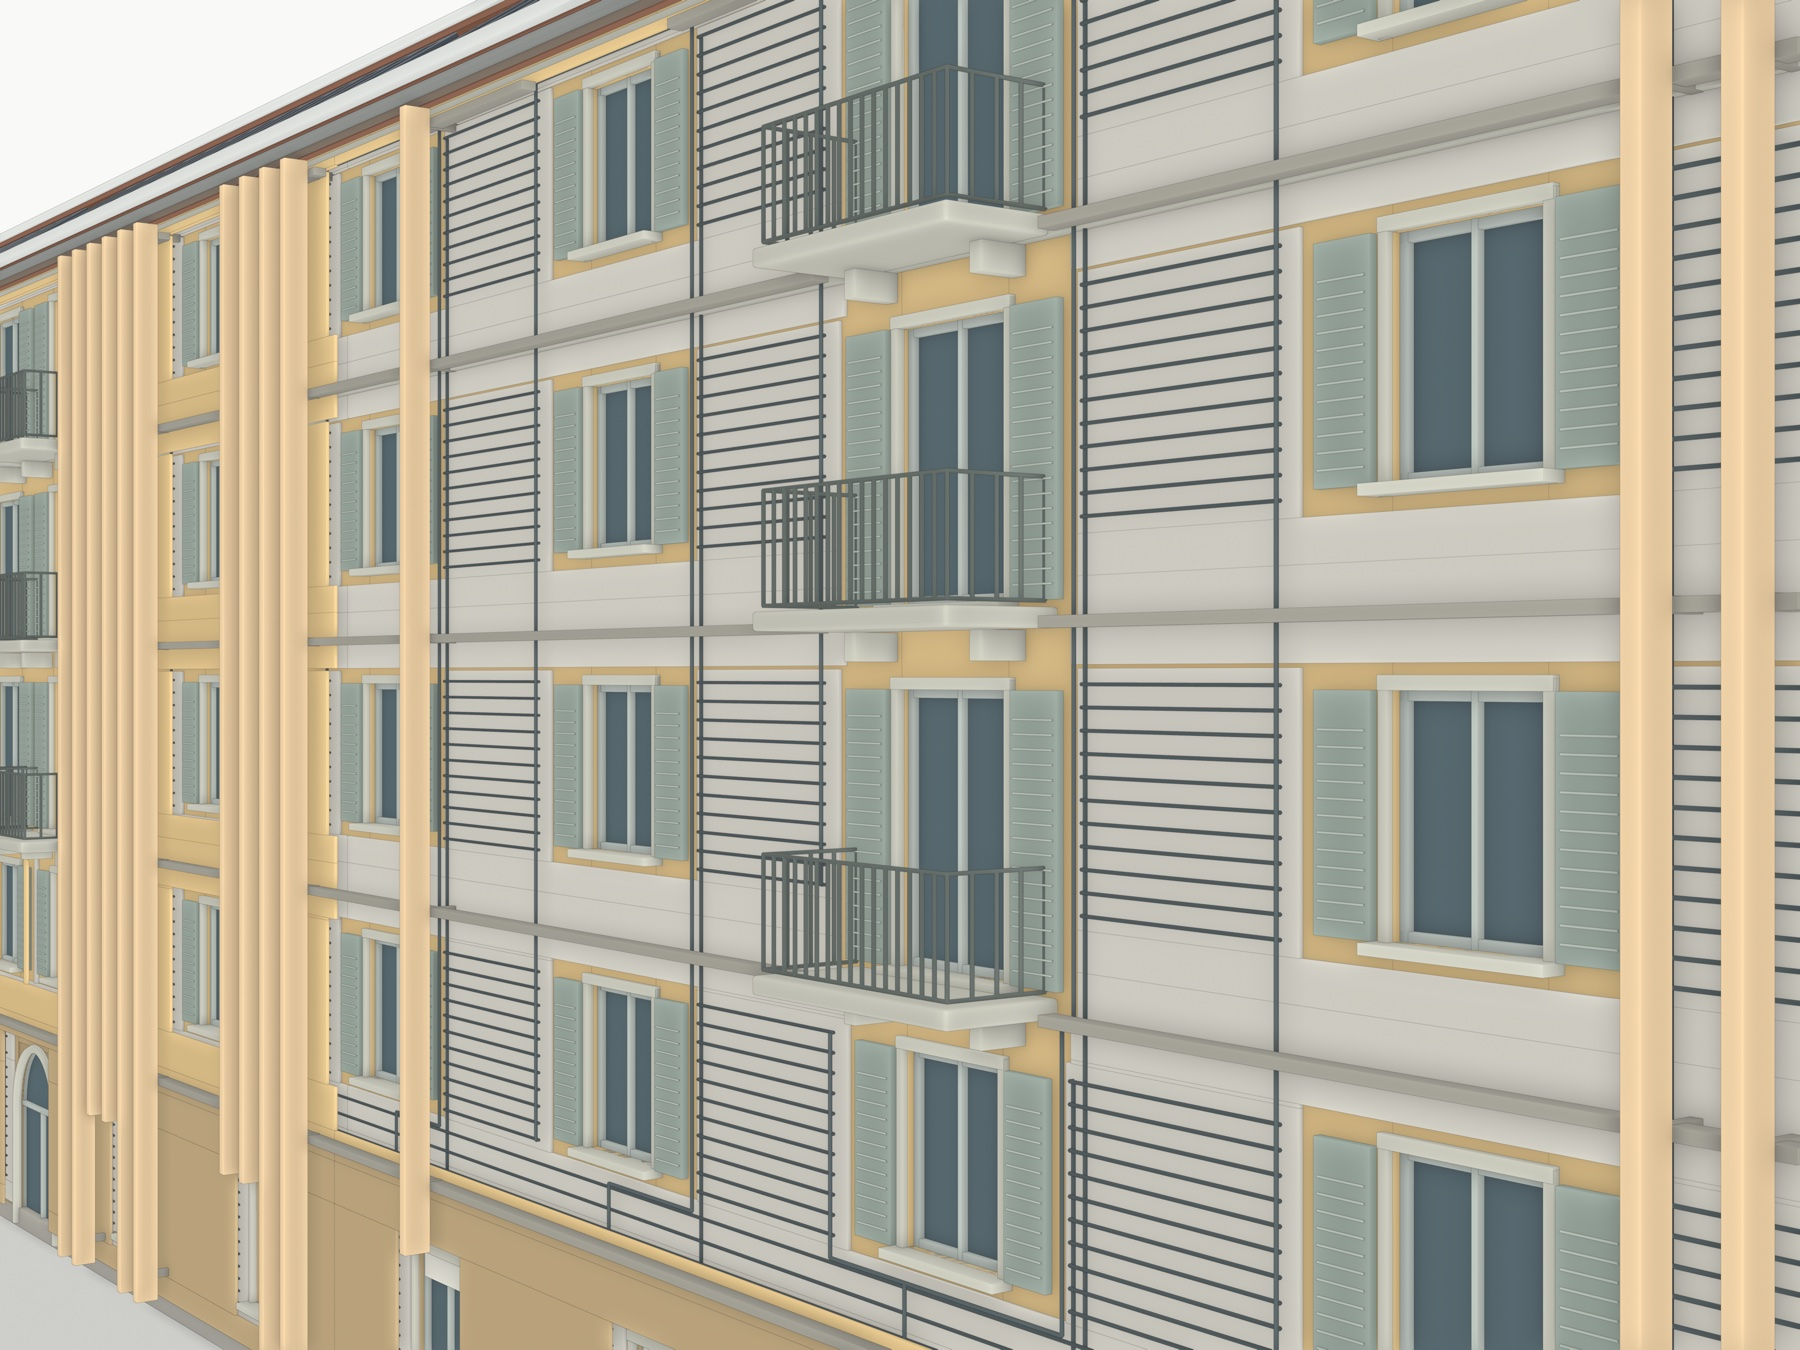
\includegraphics[width=0.85\textwidth]{figures/image15.jpg}
\caption{Pipe-access detail from our model (view 17). Parts of the covering are
removed to reveal the pipes behind the proposed separable façade panels. Render:
project team.}
\label{fig:v2access}
\end{figure}

\subsubsection{Updated Engineering Assessment}
\label{sec:v2check}

For an illustrative roof output of \qty{60}{\watt\per\square\metre}, the
\qty{740}{\square\metre} cooling area releases about \qty{44}{\kilo\watt},
supporting roughly \qty{440}{\square\metre} of façade at
\qty{100}{\watt\per\square\metre}. Repeating the circulation check with the same
height and common route gives Table~\ref{tab:pipes_v2}.

\begin{table}[!htb]
\centering
\caption{Pipe-size estimates after reducing the connected heat load.}
\label{tab:pipes_v2}
\renewcommand{\arraystretch}{1.15}
\small
\begin{tabular}{llll}
\toprule
\textbf{Water difference} & \textbf{Buoyancy pressure} & \textbf{Water flow at \qty{44}{\kilo\watt}} & \textbf{Internal diameter} \\
\midrule
\qty{10}{\celsius} (= \qty{10}{\kelvin}) & $\approx\qty{300}{\pascal}$ & $\approx\qty{1.1}{\kilo\gram\per\second}$ & $\approx\qty{120}{\milli\metre}$ \\
\qty{3}{\celsius} (= \qty{3}{\kelvin}) & $\approx\qty{90}{\pascal}$ & $\approx\qty{3.5}{\kilo\gram\per\second}$ & $\approx\qty{255}{\milli\metre}$ \\
\bottomrule
\end{tabular}
\end{table}

The drawn roof uses four long coils. Area divided by \qty{0.16}{\metre} pipe spacing
gives about $740/0.16 \approx \qty{4620}{\metre}$ of pipe, or \qty{1150}{\metre} per
coil. Assuming \qty{40}{\milli\metre} internal diameter, equal flow and a
\qty{10}{\celsius} water difference, each coil carries
$\dot m = 1.05/4 \approx \qty{0.26}{\kilo\gram\per\second}$, so
$v \approx \qty{0.21}{\metre\per\second}$, $\mathrm{Re} \approx \num{10500}$ and
$f \approx 0.031$; the Darcy equation~\eqref{eq:loss} gives
\[
\Delta p_\mathrm{coil} \approx 0.031 \cdot \frac{1150}{0.040} \cdot
\frac{996 \cdot 0.21^{2}}{2} \approx \qty{20}{\kilo\pascal}
\]
loss per coil at \qty{44}{\kilo\watt} total load, excluding bends. This exceeds the
\qty{0.30}{\kilo\pascal} buoyancy pressure by roughly a factor of 67: the long-coil
arrangement must change.

The roof and water-flow estimates prescribe temperatures separately. Water
temperature, flow and pipe-to-surface heat transfer must be solved together before
assigning an operating output.

\paragraph{A pressure budget.} A thermosiphon works only if the sum of all losses
around the loop stays below the buoyancy pressure. For the \qty{10}{\kelvin} case we
split the \qty{300}{\pascal} as follows: mains at most \qty{30}{\pascal}, roof
circuits at most \qty{60}{\pascal}, façade panels, headers and fittings at most
\qty{150}{\pascal}, and about \qty{60}{\pascal} in reserve for start-up. The mains of
Table~\ref{tab:pipes_v2} used the whole budget, so they grow: with
$\dot m = \qty{1.05}{\kilo\gram\per\second}$, $L = \qty{160}{\metre}$ and
$\Sigma K = 20$, an internal diameter of \qty{200}{\milli\metre} gives
$v \approx \qty{0.034}{\metre\per\second}$, $\mathrm{Re} \approx \num{8400}$,
$f \approx 0.033$ and a loss of about \qty{26}{\pascal}, inside the mains share.

\paragraph{Parallel roof circuits.} We keep the total roof pipe length and split it
into $N$ parallel circuits of length $L_c = \qty{4620}{\metre}/N$, each carrying
$\dot m / N$, fed from a supply header and collected by a return header. The loss per
circuit, which is the loss of the whole roof stage because the circuits are in
parallel, is
\begin{equation}
\Delta p_\mathrm{roof} = f \, \frac{L_c}{D} \, \frac{\rho v^{2}}{2},
\qquad
v = \frac{4 \dot m}{N \rho \pi D^{2}},
\qquad
f = \frac{64}{\mathrm{Re}} \ \text{for } \mathrm{Re} < 2300,
\label{eq:parallel}
\end{equation}
with the Blasius correlation above \num{2300}~\cite{white2011}. In the laminar range
$\Delta p_\mathrm{roof}$ scales with $v L_c$, so doubling $N$ divides the loss by
four. Table~\ref{tab:roofnetwork} evaluates Equation~\eqref{eq:parallel} for
$D = \qty{40}{\milli\metre}$, $\rho = \qty{996}{\kilo\gram\per\cubic\metre}$,
$\mu = \qty{0.8}{\milli\pascal\second}$ and the \qty{10}{\kelvin} flow of
\qty{1.05}{\kilo\gram\per\second}.

\begin{table}[!htb]
\centering
\caption{Roof stage as $N$ parallel circuits, \qty{40}{\milli\metre} internal
diameter, total flow \qty{1.05}{\kilo\gram\per\second} (\qty{44}{\kilo\watt} at
\qty{10}{\kelvin}). Budget for the roof stage: \qty{60}{\pascal}.}
\label{tab:roofnetwork}
\renewcommand{\arraystretch}{1.15}
\small
\begin{tabular}{rrrrrrr}
\toprule
$N$ & $L_c$ (\si{\metre}) & $\dot m$ per circuit (\si{\kilo\gram\per\second}) & $v$ (\si{\metre\per\second}) & Re & $f$ & $\Delta p_\mathrm{roof}$ (\si{\pascal}) \\
\midrule
4  & 1150 & 0.26  & 0.21   & \num{10500} & 0.031 & $\approx \num{19700}$ \\
16 & 289  & 0.066 & 0.052  & \num{2600}  & 0.044 & $\approx 440$ \\
32 & 144  & 0.033 & 0.026  & \num{1300}  & 0.049 & $\approx 60$ \\
64 & 72   & 0.016 & 0.013  & \num{650}   & 0.098 & $\approx 15$ \\
\bottomrule
\end{tabular}
\end{table}

With 32 to 64 circuits of \qtyrange{70}{145}{\metre}, the roof stage stays inside its
\qty{60}{\pascal} share, and the whole loop closes on paper: about \qty{26}{\pascal}
in the mains, \qtyrange{15}{60}{\pascal} on the roof, up to \qty{150}{\pascal} for
panels, headers and fittings, and a reserve. Two consequences follow. The flow in the
roof circuits is laminar, which lowers the heat transfer from the water to the pipe
wall and the carrier plate, so a low pressure loss is bought with a lower plate
temperature; the measured roof output asked for in Table~\ref{tab:priorities} is what
settles this. And the \qty{3}{\kelvin} case does not close with these sizes: its
\qty{3.5}{\kilo\gram\per\second} would cost about \qty{250}{\pascal} in the
\qty{200}{\milli\metre} mains alone against \qty{90}{\pascal} available. A thermosiphon
answers such a shortfall by running at a lower flow and a larger temperature
difference, and whether it starts up at all from a small difference is the first test
in Table~\ref{tab:priorities}. The long coils in Figure~\ref{fig:v2loop} are
superseded by this network; the drawing has not yet been updated.

Roof-pipe water volume is approximately
$\qty{4620}{\metre} \times \pi \times (\qty{0.04}{\metre})^{2}/4 \approx \qty{5.8}{\cubic\metre}$,
excluding façade pipes and headers, which adds about \qty{5.8}{\tonne} to the roof
load.

\paragraph{Winter operation.}
\label{sec:winter}
Before frost, the proposed circuit is emptied into storage and refilled when needed.
Drainback requires sloping pipes and air entry; Baechler and
Love~\cite[Ch.~3]{baechler2007} give about \qty{2.1}{\percent} slope. Trapped water
and pump-assisted refill remain checks~\cite{baechler2007}.

\subsubsection{Priorities for Further Development}
\label{sec:priorities}

\begin{table}[!htb]
\centering
\caption{Ranked checks needed to develop Concept V2.}
\label{tab:priorities}
\renewcommand{\arraystretch}{1.15}
\small
\begin{tabularx}{\textwidth}{L{3.2cm} X}
\toprule
\textbf{Priority} & \textbf{Check and design decision} \\
\midrule
1 Circulation & Size the parallel network including all losses (Table~\ref{tab:roofnetwork}); test start-up at small temperature differences. Decide whether buoyancy is sufficient. \\
2 Roof output & Measure heat release under varied sun, wind and sky conditions. Set the connected façade area from the result. \\
3 Winter operation & Test emptying and refill of one representative branch; measure retained water before freeze--thaw testing. \\
4 Panel assembly & Check pipe contact, leak behavior, removable connections and mounting loads. \\
5 Building and materials & Check pedestrian clearance, heritage compatibility, glare, winter gains, weathering, chemical safety and repair. \\
\bottomrule
\end{tabularx}
\end{table}
